\documentclass{beamer}

% \usepackage[latin1]{inputenc}

%% Beamer Settings

\usetheme{default}

%% Our ColorScheme
\usecolortheme{dalhousie}

%% Outer Themes - These work Nicely
\useoutertheme[height=0pt, right]{sidebar}
% \useoutertheme{split}
% \useoutertheme{miniframes}
% \useoutertheme{infolines}


%% Presentation info
\title{Design Database}
\author{Hatem Nassrat}
% \date{March 12, 2008}
\institute[2009]
{
  \deptlogo
%   Faculty of Computer Science\\
%   Dalhousie University
}


\begin{document}


%% The first way to define frames (using braces)
\frame{\titlepage}


\section[Outline]{}

\frame{\tableofcontents}


\section{Introduction}

\frame {
    \frametitle{First Frame}
    \begin{itemize}
        \item<1->One good argument
        \item<2->Another good argument, after one click
        \item<3->Last one, after another click
    \end{itemize}
}

\subsection{Example Sub Section}

\frame {
    \frametitle{Last Frame}
    This is the only frame in this subsection
}


\section{Section no.1}

%% Second Way to define Frames (using begin...end)
\begin{frame}\frametitle{Title}
  Each frame should have a title.
\end{frame}
\subsection{Subsection no.1.1  }
\begin{frame}
  Without title somethink is missing.
\end{frame}


\section{Section no. 2}

\subsection{Lists I}

\begin{frame}\frametitle{unnumbered lists}
  \begin{itemize}
    \item Introduction to  \LaTeX
    \item Course 2
    \item Termpapers and presentations with \LaTeX
    \item Beamer class
  \end{itemize}
\end{frame}

\begin{frame}\frametitle{lists with pause}
  \begin{itemize}
    \item Introduction to  \LaTeX \pause
    \item Course 2 \pause
    \item Termpapers and presentations with \LaTeX \pause
    \item Beamer class
  \end{itemize}
\end{frame}

\subsection{Lists II}

\begin{frame}\frametitle{numbered lists}
  \begin{enumerate}
    \item Introduction to  \LaTeX
    \item Course 2
    \item Termpapers and presentations with \LaTeX
    \item Beamer class
  \end{enumerate}
\end{frame}

\begin{frame}\frametitle{numbered lists with pause}
  \begin{enumerate}
    \item Introduction to  \LaTeX \pause
    \item Course 2 \pause
    \item Termpapers and presentations with \LaTeX \pause
    \item Beamer class
  \end{enumerate}
\end{frame}


\section{Section no.3}

\subsection{Tables}

\begin{frame}\frametitle{Tables}
  \begin{tabular}{|c|c|c|}
    \hline
    \textbf{Date} & \textbf{Instructor} & \textbf{Title} \\
    \hline
    WS 04/05 & Sascha Frank & First steps with  \LaTeX  \\
    \hline
    SS 05 & Sascha Frank & \LaTeX \ Course serial \\
    \hline
  \end{tabular}
\end{frame}

\begin{frame}\frametitle{Tables with pause}
  \begin{tabular}{c c c}
    A & B & C \\
    \pause
    1 & 2 & 3 \\
    \pause
    A & B & C \\
  \end{tabular}
\end{frame}


\section{Section no. 4}

\subsection{blocs}

\begin{frame}\frametitle{blocs}
  \begin{block}{title of the bloc}
    bloc text
  \end{block}
  \begin{exampleblock}{title of the bloc}
    bloc text
  \end{exampleblock}
  \begin{alertblock}{title of the bloc}
    bloc text
  \end{alertblock}
\end{frame}


\section{Section no. 5}

\subsection{split screen}

\begin{frame}\frametitle{splitting screen}
  \begin{columns}
    \begin{column}{4cm}
      \begin{itemize}
        \item Beamer
        \item Beamer Class
        \item Beamer Class Latex
      \end{itemize}
    \end{column}
    \begin{column}{5cm}
      \begin{tabular}{|c|c|}
        \hline
        \textbf{Instructor} & \textbf{Title} \\
        \hline
        Sascha Frank &  Course 1 \\
        \hline
        Sascha Frank &  Course serial  \\
        \hline
      \end{tabular}
    \end{column}
  \end{columns}
\end{frame}

\subsection{Pictures}

\begin{frame}\frametitle{pictures in latex beamer class}
  \begin{figure}
    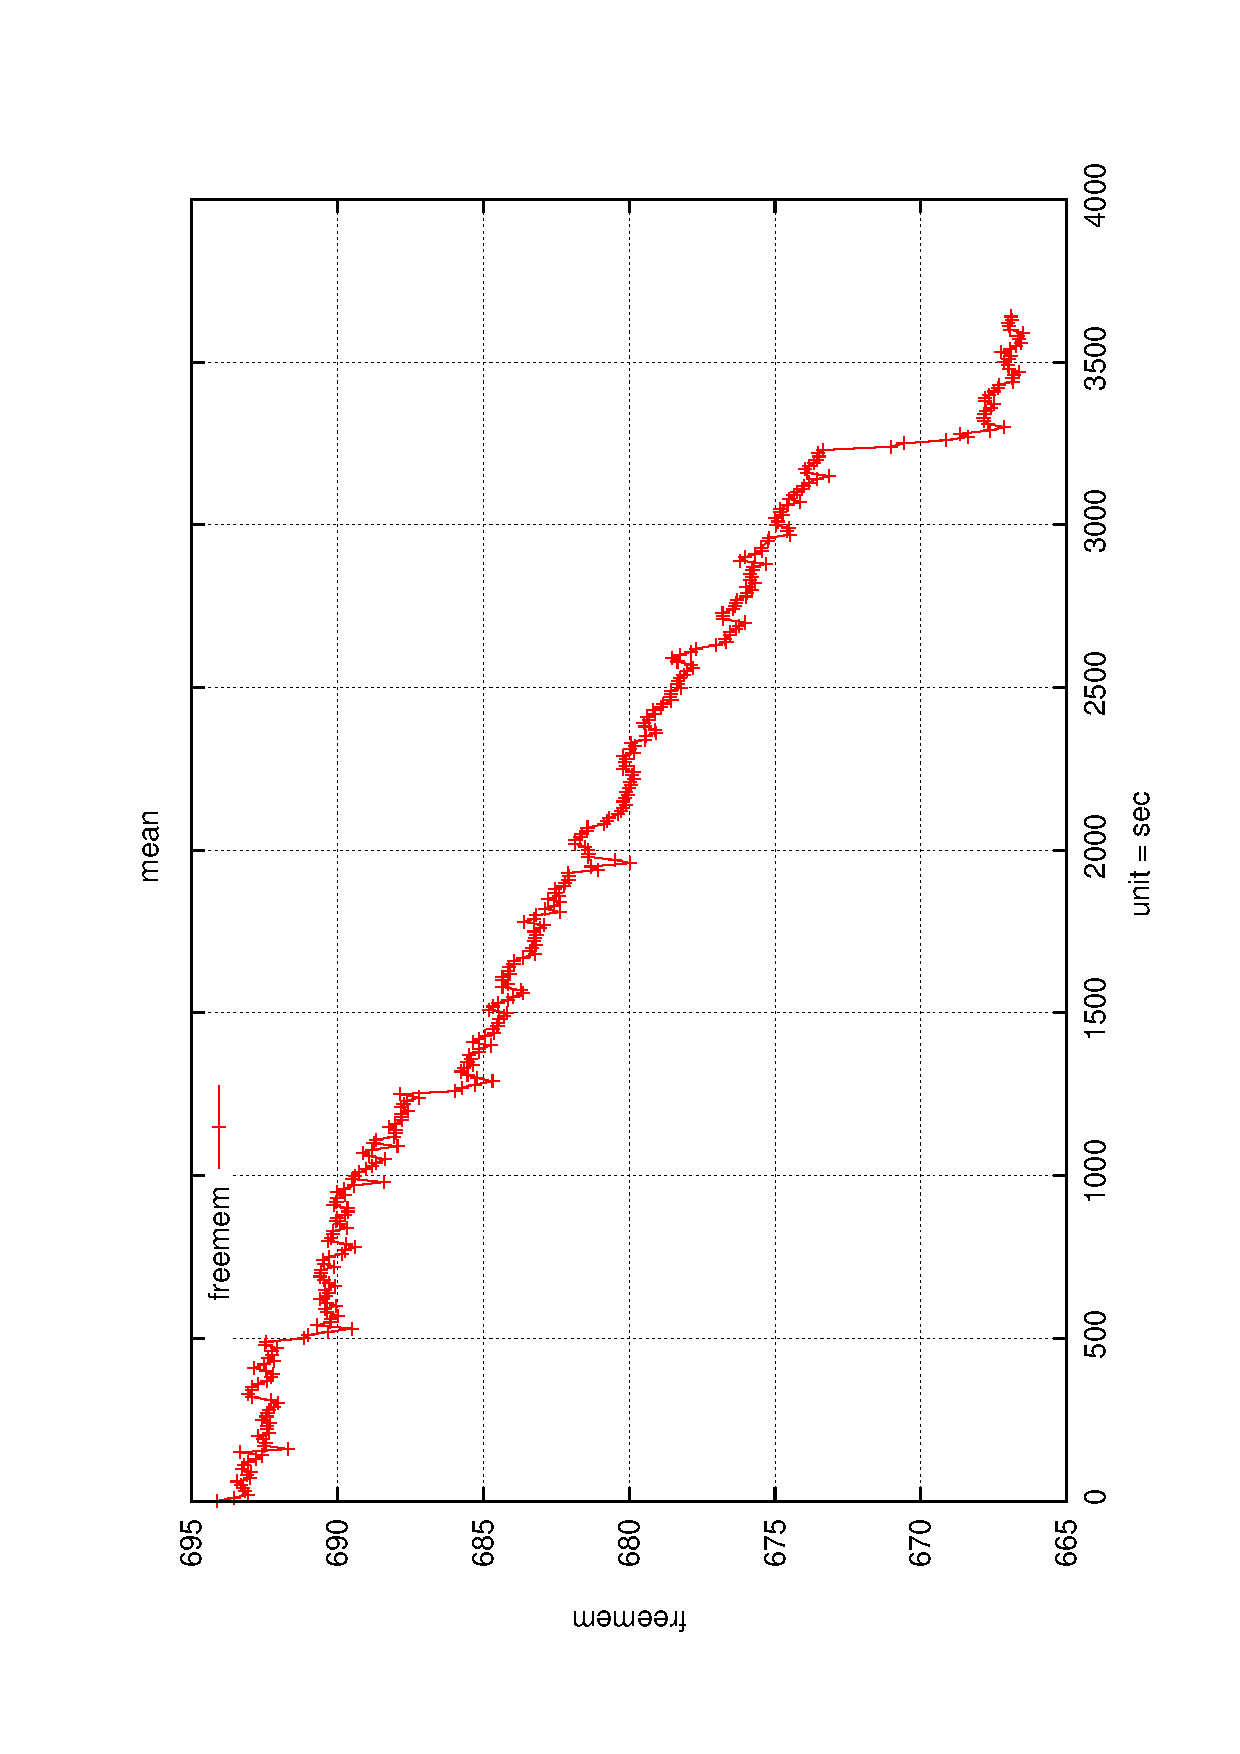
\includegraphics[width=2in, angle=-90]{figs/PIC1}
    \caption{show an example graphic}
  \end{figure}
\end{frame}

\subsection{joining picture and lists}

\begin{frame}
  \frametitle{pictures and lists in beamer class}
  \begin{columns}
    \begin{column}{4cm}
      \begin{itemize}
        \item<1-> subject 1
        \item<3-> subject 2
        \item<5-> subject 3
      \end{itemize}
      \vspace{3cm}
    \end{column}
    \begin{column}{5cm}
      \begin{overprint}
        \includegraphics<2>[width=1.5in, angle=-90]{figs/PIC1}
        \includegraphics<4>[width=1.5in, angle=-90]{figs/PIC2}
        \includegraphics<6>[width=1.5in, angle=-90]{figs/PIC3}
      \end{overprint}
    \end{column}
  \end{columns}
\end{frame}

\subsection{pictures which need more space}

\begin{frame}[plain]
  \frametitle{plain, or a way to get more space}
  \begin{figure}
    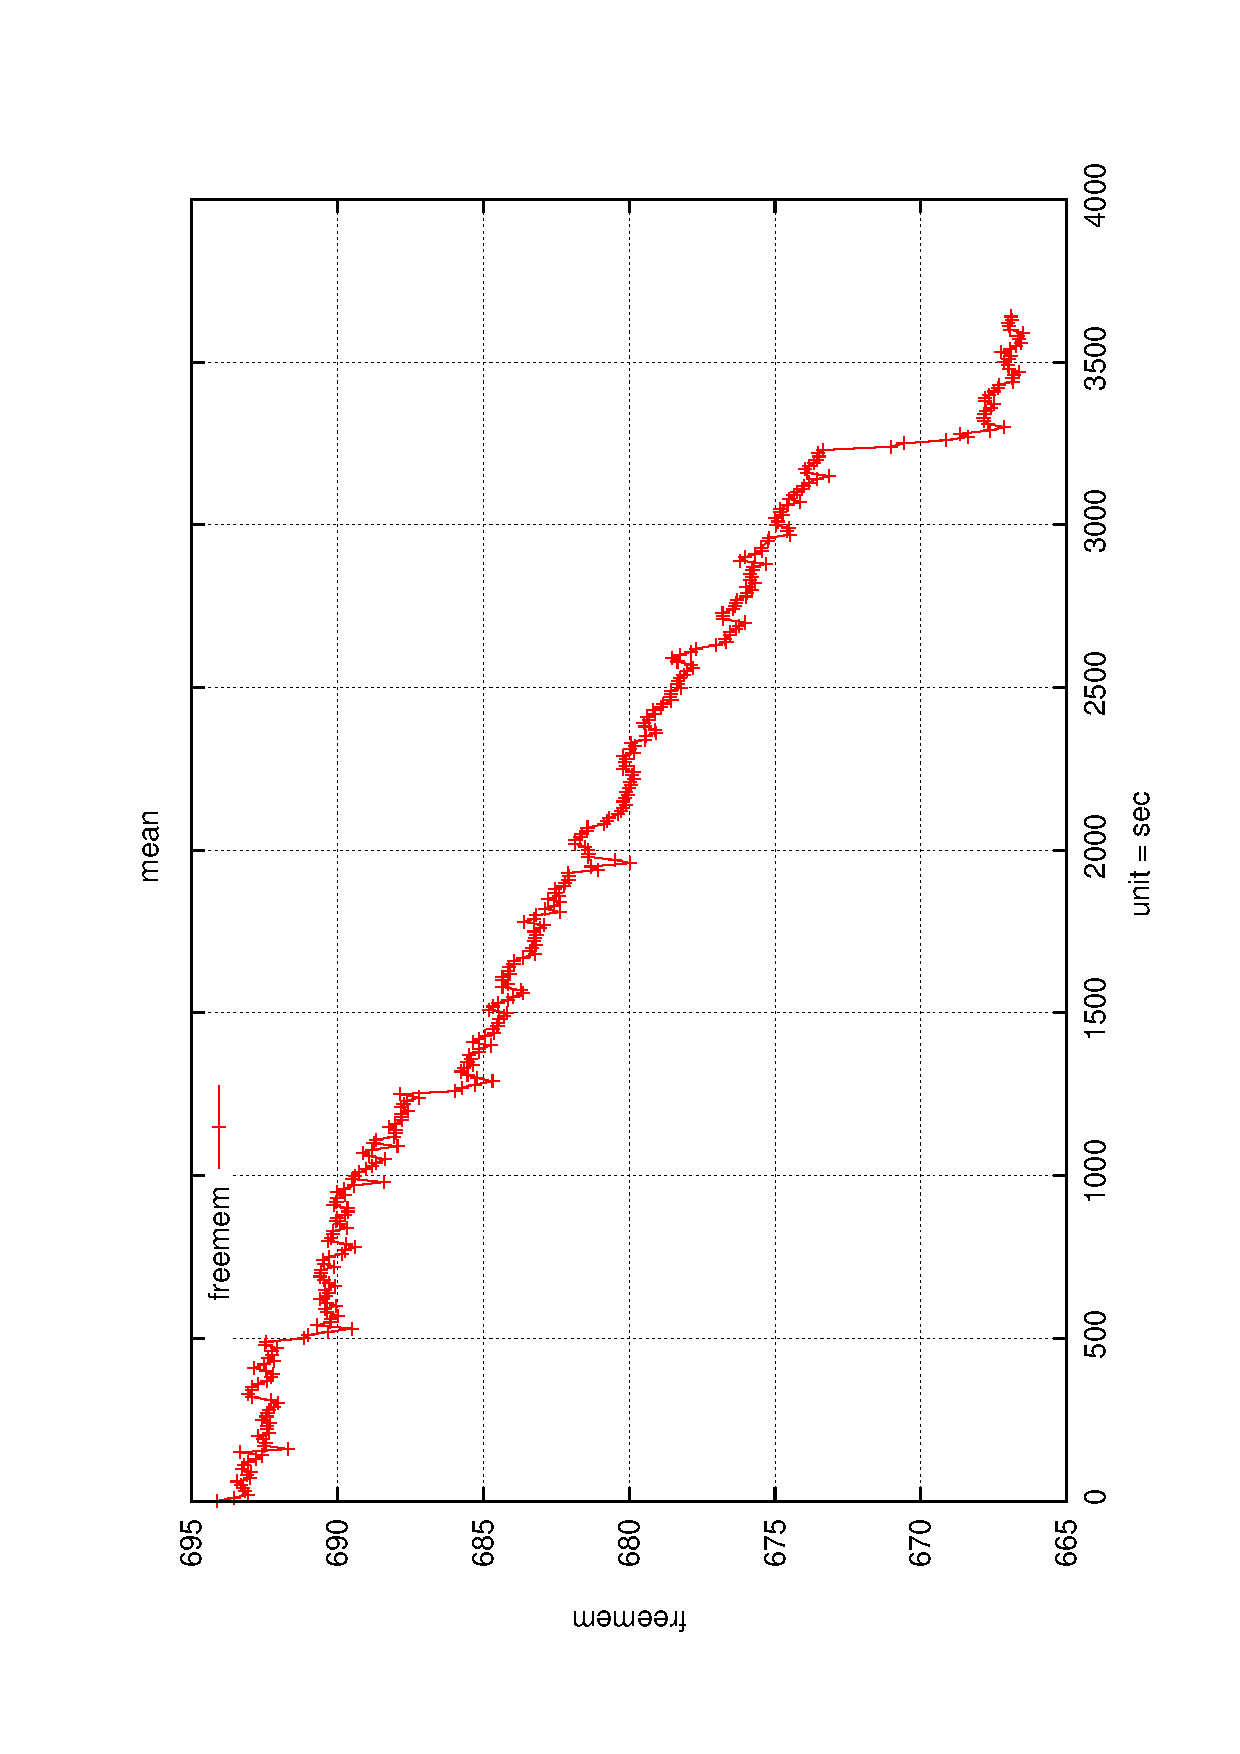
\includegraphics[width=2.7in, height=4.5in, angle=-90]{figs/PIC1}
    \caption{show an example picture}
  \end{figure}
\end{frame}


\appendix

\section<presentation>*{\appendixname}

\subsection<presentation>{For Further Reading}

\begin{frame}[allowframebreaks]
  \frametitle<presentation>{For Further Reading}

  \begin{thebibliography}{10}

  \beamertemplatebookbibitems
  % Start with overview books.

  \bibitem{Author1990}
    A.~Author.
    \newblock {\em Handbook of Everything}.
    \newblock Some Press, 1990.

  \beamertemplatearticlebibitems
  % Followed by interesting articles. Keep the list short.

  \bibitem{Someone2000}
    S.~Someone.
    \newblock On this and that.
    \newblock {\em Journal of This and That}, 2(1):50--100,
    2000.
  \end{thebibliography}
\end{frame}

\end{document}

% vim: sw=2:
